% !TEX root = mythesis.tex

%==============================================================================
\chapter{Interpolating Operators}
\label{sec:ops}
%==============================================================================

The overarching aim of hadron spectroscopy on the lattice is to simulate hadrons that we observe in collider experiments. It is advantageous in lattice QCD studies to generate a large basis of interpolating operators to achieve maximal overlap with energy levels of interest. Distillation allows us to restrict this basis to maximize computational efficiency in both the generation of the fundamental objects (perambulators, elementals) and contractions. We first focus on the zero momentum case then extend this framework to non-zero momentum, eg. mesons in flight. We need to construct operators with the flavor basis $\bar c\bar s ud$, $c\bar s u\bar d$, $cc\bar u\bar d$ and $c\bar c u\bar d$, which create and destory a mesonic state, at some fixed time in Euclidean time. The destruction of the state is executed via a contraction of the creation operator with its adjoint at some later time $t$.  The information we can glean from this is the correlation of operators separated by some time $t$, whereby the transfer matrix eigenstates can be obtained. Moreover, the key difference between lattice and continuum eigenstates is the notion of spin, thus we must work in the circular basis of cartesian-vector-like derivative operators and gamma matrices \cite{Morningstar:2013bda}. Using the preceeding section on correlator function construction from contractions, here we will form local and non-local distilled bilinear operators in different irreps of $O_h$, which will comprise a $N \times N$ matrix of two-point correlation functions for each irrep, the GEVP. The dimension of this matrix is, not surprisingly, the number of operators constructed in the particular irrep, as we cannot mix operators with different continuum quantum numbers. Our test case will be $J^{PC} =0^{-+}$, e.g. a pseudoscalar such as the pion. We will walk through lattice operator construction to create a diqaurk $[\bar{q}q]$ of any spin ($J \in \mathbb{Z}$) and parity $P$ with two quark fields and an insertion of the covariant derivative $\nabla$ with gamma strucutre $\Gamma$, the product of which determines the spin $J$.  
  

\section{Spin on a cubic lattice}
Angular momentum ceases to be a good quantum number on the lattice. Thus, in order to forge a link between conntinuum spin and spin on the lattice, we must transform lattice operators according to irreps of the cubic group $O_h$. This optimizes the signal to noise ratio. Only then can we extract eigenstates of the hamiltonian. The lattice irreps, representing symmetries of the cube, are
\begin{align}
    \Lambda = {A_1,T_1,T_2,E,A_2}
\end{align}
\begin{table}
    \begin{tabular}{ccc}
    $\Lambda$ & $d_{\Lambda}$ & $J$\\ \hline
    $A_1$ & 1 & $0,4,6,\dots$\\
    $A_2$ & 1 & $3,6,7,\dots$\\
    $E$ & 2 & $2,4,5,\dots$\\
    $T_1$ & 3 & $1,3,4,\dots$\\
    $T_2$ & 3 & $2,3,4,\dots$\\ \hline
    \end{tabular}
    \caption{The table shows the single-valued irreducible representations
      $\Lambda$ of the cubic group $O$, together with their dimensions
      $d_\Lambda$ and continuum spin content $J$\protect.\label{tab:irrep}}
    \end{table}

\section{Operators on the lattice}
A hadronic operator is a functional of the lattice fields with supplied quantum numbers. These are the gauge-invariant color singlet objects. The lattice regulator ``breaks'' the $SO(3)$ subgroup to a discrete subgroup. $O,\bar{O}$ mapped into the appropiate Hilbert Space such that the corresponding operators $\hat{O} ,\hat{O^\dagger}$  annihilate and create the particle states of interest. We can identify physically allowed states via the spectral decomposition of propagators of interpolating operators: 
\begin{equation}
\braket{O(n_t)\bar{O(0)}} = \sum_{n}\braket{0|\hat{O}|k} \braket{k|\hat{O^{\dagger}}|0} e^{-n_taE_k}
\end{equation}

It is important to note that different spin and parity correspond to different gamma matrices in the fermionic bilinears. Armed with the continuum version of operators, which are classified via charge conjugation and Lorentz transformations, we can cosntruct our lattice operators. The first step is to perform a Wick rotation so that our operators now reside in euclidean spacetime, then substitute the covariant derivatives with the lattice covariant derivative \cite{G_ckeler_1996}, 
\begin{align}
    \overrightarrow{D_\mu}\psi(x) = \frac{1}{2a}(U_{x,\mu}\psi(x + \hat{\mu}) - U_{x-\hat{\mu},\mu}^\dagger\psi(x - \hat{\mu}))
\end{align}

\section{Meson operators at zero total momentum}
We detail the operator construction for zero total momentum, continuum spin $J^P$ and spin component $m$. In general, a local meson interpolator has the form $O_M(n) = \bar{\psi}^{f_1}(n)\Gamma\psi^{f_2}(n)$ where $\Gamma$ is a monomial of gamma matrices and $f$ are of the exposed flavor indices. In our calculations, the fermions fields $\bar{\psi},\psi$ are smeared with the distillation operator. The ingredients are gauge-covariant derivatives(for local operators this is just $\mathbb{I}$), Dirac matrix $\Gamma$, and the distilled meson elementals and perambulators. We obtain the lattice interpolator from the general(continuum) operator by subducing into irreps of the octahedral group $O_h$. 

% In table 1 of \cite{Cheung_2017}, we have the following for the 0 total momentum states: 
% \begin{table}
%     \begin{tabular}{ccc}
%     $LG$ & $\Lambda^p$ & $J^p$ \\
%     \hline
%     $O_h$ & $T_1^+$ & $1^+$ \\
%     $O_h$ & $A_1^-$ & $0^-$ \\
% \end{tabular}
% \end{table}
Fermion-bilinear operators with continuum spin $J$ and momentum $\vec{p}$ are written like so \cite{Cheung_2017}
    \begin{equation}
    \mathcal{O}^{J,m}(\vec{p},t) = \sum_{\vec{x}} e^{i\vec{p}\vec{x}} \bar{q}(\vec{x},t) [\Gamma \overleftrightarrow{D}\dots \overleftrightarrow{D}]^{J,m}q(\vec{x},t)
\end{equation}
In the most general form,

\begin{equation}
    \mathcal{O}_{\Lambda,\mu}^P(\vec{p}=\vec{0},t) = \sum_{\mu_1,\mu_2,\hat{q}} \mathbb{C}(\vec{p} = \vec{0},\Lambda^P,\mu;\vec{q},\Lambda_1,\mu_1;-\vec{q},\Lambda_2,\mu_2) \Omega^{M_1}_{\Lambda_1,\mu_1}(\vec{q},t) \Omega^{M_2}_{\Lambda_2,\mu_2}(-\vec{q},t)
\end{equation}

\section{Local meson operators}

The simplest interpolating operators are the local fermion bilinears $\bar{\psi}(x)\Gamma\psi(x)$. These are preferred as their corresponding gamma structure is much simpler to implement in the contractions. Local signifies that the quark fields at the source and sink are not spatially displaced on gauge links. However, the only continuum quantum numbers we can access with local operators are $J^{PC} = 0^{-+},0^{++},1^{++},1^{+-},1^{--}$ \cite{Dudek_2008}.

For the single pion case, the gamma structure to be inserted between the elementals and perambulators at times $t_0,t_f$, forming the fermion bilinear are
\begin{itemize}
    \item $\gamma_4\gamma_5$
    \item $\gamma_5$

\end{itemize}

\section{Nonlocal meson operators}
To study orbitally excited mesons (higher spin states) we need to employ derivative operators which characterize spatial displacement of quarks on the lattice. These ``forward-backward" gauge covariant derivatives allow us to access states with higher angular momentum. On the lattice, these derivatives are finite displacements of quark fields connected by the gauge links. We will include zero, single, and double derivative operators. We must ensure that the operators have definite charge conjugation as well as a projection operator within the corresponding irreps \cite{liao2002excitedcharmoniumspectrumanisotropic}. Our simplest operator, representing a gauge-invariant construction of a quark and antiquark located at different sites on the lattice along some path $P$ is 
\begin{align}
    \tilde{\psi}_(x_2)\Pi_P U \Gamma \psi(x_1)
\end{align}
where $\Gamma$ takes one of the following forms depending on the state of interest. To access the $J^{PC}=0^{-+}$ channel, we have a set of three pseudoscalar operators which we can then solve the GEVP for

\begin{tabular}{ccc}
    op. & name & cont. \\
    \hline
    $\gamma^i \mathbb{B}^i$ & $(\rho \times \mathbb{B})_{A_1}$ & $0^{-+}$ \\
    $\gamma^4 \gamma^i \mathbb{B}^i$ & $(\rho_{(2)} \times \mathbb{B})_{A_1}$ & $0^{-+}$ \\
    $\gamma^4 \gamma^5 \gamma^i \nabla^i$ & $(b_1 \times \nabla)_{A_1}$ & $0^{-+}$ \\
    \end{tabular}

The advantage of employing nonlocal operators is to achieve access to states with nonzero orbital angular momentum. We act on local meson operators with gauge covariant lattice displacements on one (source or sink) or both (source and sink), the smeared quark fields of the discretized theory, to produce nonlocal operators. 

\subsection{Derivative operators}
Parallel transport of a lattice field is performed by applying a displacement operator to a quark field.  Let $q(x)$ be a quark field and $D_j^{(p)}$ ai displacement operator that moves the quark field for p lattice sites to the direction j in a covariant manner. Let $U$ be the gauge-link as defined in the previous section.
\begin{align}
    D_j^{(p)} q(x) = U_j(x) U_j(x+j) U_j(x+2j)...U_j(x+(p-1)j) q(x+pj)
\end{align}
with dictionary $x(0), y(1), z(2)$.

Thus, a quark bilinear in its $O_h$ representation is tied together with the spatial path $(x_1 \to x_2$). Our new operator will thus live in a representation determined by the Clebsch-Gordan decomposition of the product of representations \cite{Basak_2005}. The set of operators must have definite charge conjugation and the correct projection operator such that it resides in the proper irrep of the cubic group as dictated by group theory.  

\subsubsection{Single derivative operators}
The general form for single derivative meson operators, in which operators of definite spin can be constructed using the standard $SO(3)$ Clebsch-Gordan coefficients, e.g. for a vector-like gamma matrix and one covariant derivative, operators of $J=0,1,2$ can be formed \cite{Dudek_2010}
\begin{equation}
 (\Gamma \times D^{[1]}_{J=1} )^{J, M} = \sum_{m_1, m_2}\big\langle 1, m_1 ; 1, m_2 \big| J, M
  \big\rangle\,  \bar{\psi} \Gamma_{m_1}
  \overleftrightarrow{D}_{m_2} \psi. \nonumber
\end{equation}
The choice of $\Gamma$ plays a role in setting the parity and charge-conjugation quantum numbers of the operator, where the typical naming convention is given by the lowest lying meson in that particular channel. As noted in the introduction of this chapter, we must distribute the different $M$ components belonging to a meson of spin $J$ into definite cubic(lattice) irreps via the group theoretical process called subduction. This is carried out by linear combinations of the $M$ components for each $J$\cite{Dudek_2010}:
\begin{eqnarray}
{\cal O}^{[J]}_{\Lambda,\lambda} \equiv (\Gamma \times D^{[n_D]}_{\ldots})^J_{\Lambda, \lambda} =  \nonumber\\
& & \sum_M {\cal
     S}^{J,M}_{\Lambda, \lambda}   \; (\Gamma \times
   D^{[n_D]}_{\ldots})^{J,M} \equiv \sum_M {\cal S}^{J,M}_{\Lambda,\lambda} {\cal O}^{J,M}, \nonumber
\end{eqnarray}
where $\lambda$ is the ``row'' of the irrep ($1\ldots\mathrm{dim}(\Lambda)$). 

% \subsubsection{Example for $J=0$}
% As seen in the appendix, since this spin value only subduces into the $A_1$ irrep, $\cal{S}_{A1,1}^{0,0} = 1$. This coefficient would correspond to \todo{example state and operator}

%-------------------------------------------------------------------------------%

\subsubsection{Two derivative operators}

\begin{tabular}{|c|c|}
    \hline
    Operator & Lattice spatial displacement correspondence\\
    \hline
    $\gamma_5 \mathbb{D}^i$ & $[\gamma_5 * (dydz + dzdy), \gamma_5 * (dzdx + dxdz), \gamma_5 * (dxdy + dydx)]$ \\
    \hline
    $\gamma_4 \gamma_5 \mathbb{D}^i$ & $[\gamma_5\gamma_4 * (dydz + dzdy), \gamma_5\gamma_4 * (dzdx + dxdz), \gamma_5\gamma_4 * (dxdy + dydx)]$ \\
    \hline
    $\gamma_5 \mathbb{B}^i$ & $[\gamma_5 * (dydz + -dzdy), \gamma_5 * (dzdx + -dxdz), \gamma_5 * (dxdy + -dydx)]$ \\
    \hline
    $\gamma_4 \gamma_5 \mathbb{B}^i$ & $[\gamma_5\gamma_4 * (dydz + -dzdy), \gamma_5\gamma_4 * (dzdx + -dxdz), \gamma_5\gamma_4 * (dxdy + -dydx)]$ \\
    \hline
    % $\gamma_5 \mathbb{E}^i$ & Correspondence not specified \\
    % \hline
    % $\gamma_4 \gamma_5 \mathbb{E}^i$ & Correspondence not specified \\
    % \hline
\end{tabular}


\subsubsection{Momentum projection}
Although we have not yet implemented non-zero momentum into our analysis suite, we very briefly describe what it will entail \cite{Ueding_thesis}. For non-local operators used to construct mesons in flight, we must ``momentum project" into states of definite momentum, which will reside in some irreducible representation of the octahedral group. We want mesonic states to possess definite spatial momentum on each time slice. Note that it is only necessary to project one of the two interpolators of a correlation function to definite momentum, typically at the sink.
$\tilde{O}(\textbf{p},n_t) = \frac{1}{\sqrt{\Lambda_3}} \sum_{n\in\Lambda_3} O(\textbf{n},nt)e^{-ia\textbf{np}}$ 
At non-zero momentum, $O_h$ is broken down to the little groups of Dicyclic nature, eg. $DiC_2, DiC_4$. The extra ingredient required, in contrast to the zero momentum operators, are subduction coefficients that define the helicity operators. For these, we use the Wigner D-matrices then subduce into the irreps of the little group corresponding to the little group of the total momentum $\vec{P}$. See \cite{Basak_2005},\cite{morningstar_extended_2013} for further information. The crucial piece is that these interpolators for mesons in flight will be put into the GEVP for every relevant irrep. 

\section{Meson-Meson Interpolators}
The global $SU(3)$ color symmetry requires that the minimal irreducible color singlet systems can only be $q\bar{q}$, $qqq$, $gg$, $q\bar{q}g$ etc., which implies that multi-quark systems can only exist as molecular configurations if there are no other binding mechanisms \cite{Abolnikov:2024key}. Moreover, as a consequence of the $SU(3)^C$ coupling rule, the state $QQ\bar{q}\bar{q}$ has a dimeson configuration as well as a diquark-antidiquark configuration \cite{Brambilla:2019esw}\cite{Padmanath_2022}. Due to the $SU(3)_c$ coupling rule, when treating tetraquarks as a dimeson system, $(q\bar{q})(q\bar{q})$, the two possible combinations of dimeson $SU(3)_c$ representations that produce a total color singlet state are $({1_c \otimes 1_c})_{1_c}$ and $({8_c \otimes 8_c})_{1_c}$\cite{Guo:2017jvc}. When the pseudoscalar $D$ and vector $D^*$ are coupled together, the resulting system is $DD^*$ with total angular momentum and parity $J^P = 1^+$. Moreover, the wave function of the tetraquark state $T_{cc}^+$ includes two color singlet channels:
\begin{align}
    DD^* = \frac{1}{\sqrt{2}}(D^{0*}D^+ - D^+D^*), \\
    D^*D^* = \frac{1}{\sqrt{2}}(D^{*0}D^{*+} - D^{*+}D^{*0})
\end{align} 
Meson-meson operators are constructed out of single-meson elementals. For mesons in flight, we need to access the helicity operators.  

In general, \textbf{meson-meson operators} are constructed by forming a product of two single-meson operators with appropriate flavor symmetry: \cite{Junnarkar_2019}
\begin{align}
\mathcal{M}^1(x) &= M_1(x)M_2^*(x) - M_2(x)M_1^*(x) \\
M_{1,2}(x) &= (l_{1,2})^a_\alpha(x) (\gamma_5)_{\alpha\beta} \bar{Q}^a_\beta(x) \\
M_{1,2}^*(x) &= (l_{1,2})^a_\alpha(x) (\gamma_i)_{\alpha\beta} \bar{Q}^a_\beta(x) 
\end{align}

Fermion-bilinear operators with continuum spin $J$ and momentum $\vec{p}$ are written like so \cite{Cheung_2017}
\begin{equation}
\mathcal{O}^{J,m}(\vec{p},t) = \sum_{\vec{x}} e^{i\vec{p}\vec{x}} \bar{q}(\vec{x},t) [\Gamma \overleftrightarrow{D}\dots \overleftrightarrow{D}]^{J,m}q(\vec{x},t)\
\end{equation}
% In the most general form,

% \begin{equation}
%     \mathcal{O}_{\Lambda,\mu}^P(\vec{p}=\vec{0},t) = \sum_{\mu_1,\mu_2,\hat{q}} \mathbb{C}(\vec{p} = \vec{0},\Lambda^P,\mu;\vec{q},\Lambda_1,\mu_1;-\vec{q},\Lambda_2,\mu_2) \Omega^{M_1}_{\Lambda_1,\mu_1}(\vec{q},t) \Omega^{M_2}_{\Lambda_2,\mu_2}(-\vec{q},t)
% \end{equation}
% \newpage
% The interpolators we will consider follow that of ~\cite{Padmanath_2022} in Table I, 
\begin{figure}
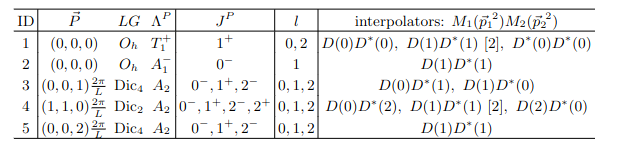
\includegraphics[scale=0.6]{interpolator_table.png}\
\caption{Interpolators along with their total momenta, spatial lattice symmetry group, total spin-parity, and partial wave (of $DD^*$ scattering) that contribute to each irreducible representation}
\end{figure}
\subsection{Distilled Meson-Meson Interpolators}
First, consider the creation and annihilation interpolators for the \(D(0)\) meson with quark content \(c\bar{u}\), \(\bar{c}u\). For smeared quark sources, we can write \cite{peardon_novel_2009} 
\begin{align}
    O(x_0,t_0) &= \Bigg[\sum_{x_1} S_i^{t_0,\alpha_0,a_0}(x_1)^{\alpha_1}_{a_1}\bar{q}^{(f)}(x_1,t)^{\alpha_1}_{a_1}\Bigg] \Gamma^{\alpha_0\beta_0} \Bigg[\sum_{x_2} (S_k^{t_0,\beta_0,a_0}(x_2)^\dagger)^{\alpha_2}_{a_2}\bar{q}^{(f')}(x_2,t)^{\alpha_2}_{a_2}\Bigg] \\
    &= \overline{q_i}(x_0, t)^{\alpha_0}_{a_0} \Gamma^{\alpha_0\beta_0} q_k(x_0,t)^{\beta_0}_{a_0}
\end{align}

Let \(S = \Box\) and Fourier transform into \(p\)-space. 
\[
\overline{\chi}(p, t) = \overline{u}_w(t) \Box_{wx}(t) \cdot e^{-ip\cdot x} \Gamma^A_{xy}(t) \cdot \Box_{yz}(t) c_z(t)
\]

Simplifying the notation (e.g., \(\Gamma^A = e^{-ip\cdot x} \Gamma^A_{xy}(t)\)), we can express the correlation function as 
\begin{align}
C^{2\text{-pt}}(t^\prime, t) &= \braket{\chi(t) \overline{\chi}(t^\prime)} \\
&= \braket{
\overline{c}(t^\prime) \Box(t^\prime) \Gamma^B(t^\prime) \Box(t^\prime) u(t^\prime) \cdot
\overline{u}(t) \Box(t) \Gamma^A(t) \Box(t) c(t)
} \\ 
&= \text{Tr}\left[
    \overline{u}(t^\prime) V(t^\prime) \cdot 
    \underbrace{V^\dagger(t^\prime) \Gamma^B V(t^\prime)}_{\Phi^B(t^\prime)} \cdot 
    V^\dagger(t^\prime) c(t^\prime) \cdot 
    \overline{c}(t) V(t) \cdot 
    \underbrace{V^\dagger(t) \Gamma^A V(t)}_{\Phi^A(t)} \cdot 
    V^\dagger(t) u(t)
\right] \\
&= \text{Tr} \left[\Phi^B(t^\prime) \cdot 
    \underbrace{V^\dagger(t^\prime) c(t^\prime) \overline{c}(t) V(t)}_{\tau_c(t^\prime, t)} \cdot 
    \Phi^A(t) \cdot 
    \underbrace{V^\dagger(t) u(t) \overline{u}(t^\prime) V(t^\prime)}_{\tau_u(t, t^\prime)}
\right] \\
&= \text{Tr}\left[\Phi^A(t) \tau_u(t^\prime, t) \Phi^B(t) \tau_c(t, t^\prime)\right]
\end{align}

Here we have defined the \textbf{perambulator} (including Dirac indices)

\begin{equation}
\tau_q(t^\prime, t)^{\alpha \beta} = V^\dagger(t^\prime) D^{-1}_q(t^\prime, t)^{\alpha \beta} V(t)
\end{equation}

as well as elemental $\Phi$
    
\begin{align}
\Phi^{A, \alpha\beta} 
&= V^\dagger(t) (\Gamma^A)^{\alpha \beta} V(t) \\
&= V^\dagger(t) \mathcal D^A(t)V(t) \mathcal S^{A, \alpha \beta}
\end{align}

where in the second line we have assumed we can decompose \(\Phi\) into terms that act only within coordinate/color space \(\mathcal{D}\) or Dirac spin space \(\mathcal{S}\).

\subsubsection{Distilled Meson-Meson Correlators}
Wick's theorem says that a correlation function is given by the sum of all possible pairs of quark contractions, specifically batched tensor contractions. Given a dimeson operator $[MM']$, we have the following spectral decomposition: 
\begin{align}
    \braket{[MM'](t) [MM']^\dagger(0)} = \sum_{n}^{} |Z_{MM'}^{(n)}|^2 e^{-E_{MM'}^{(n)}t}
\end{align}

As described in the chapter on operator construction, we can form a set of $N$ $MM'$ interpolating operators $$\{[MM']^{(0)},\dots,[MM']^{(N)}\}$$ which have non-trivial overlap with the mesonic state of interest $MM'$. The question is thus, how does one determine the magnitude of the overlaps with the state of interest? Conveniently, the outer product of the set of $N$ interpolating operators acting on itself creates a $N \times N$ matrix of $MM'$ correlators. Not surprisingly, these share the same spectrum. 

In theory, one could fit all $N \times N$ correlators using a simultaneous fit, however, at this point it is standard practice to solve the generalized eigenvalue problem for the set of correlation functions. Solving the following for the eigenvectors $v_n(t,t_0)$ gives us an optimized operator basis
\begin{align}
    C(t)v_n(t,t_0) = \lambda_n(t,t_0)C(t_0)v_n(t,t_0)
\end{align}
Instead of solving the GEVP at the operator level, we deal with the correlation functions directly to yield the optimized correlators 
\begin{align}
    \braket{[MM'](t) [MM']^\dagger(0)} = \sum_{n}^{} |Z_{MM'}^{(n)}|^2 e^{-E_{MM'}^{(n)}t} 
\end{align}

